\section{Physical Quantities}

\subsection{units of measurement}

any physical quantity contains a numerical value and its associated unit

a system of units of measurement used throughout the scientific world is the \keypoint{SI units}\index{SI unit}\footnote{SI units, abbreviated from the French \emph{Syst\`eme Internationale d'Unit\'es}, means the International System of Units. Those who are interested in the history and evolution of the SI can check out the Wikipedia article: \url{https://en.wikipedia.org/wiki/International_System_of_Units}}

\subsubsection{SI base units}

SI defines seven units of measure as a basic set, known as the \keypoint{SI base units}

\begin{center}
	\begin{tabular}{|C{5.4cm}|C{3cm}|C{3cm}|}
		\hline base quantity & base unit & symbol  \\ 
		\hline mass  & kilogram & kg \\ 
		\hline length & metre & m \\ 
		\hline time & second & s \\ 
		\hline electric current  & ampere & A \\ 
		\hline temperature & kelvin & K \\ 
		\hline amount of substance & mole & mol \\ 
		\hline luminous intensity & candela & cd \\ 
		\hline 
	\end{tabular} 
\end{center}


\subsubsection{derived units}

the seven\footnote{Luminous intensity is beyond the scope of the AS-Level syllabus. You are only required to know the other six SI base quantities and their units.} SI base units are building blocks of the SI system

all other quantities are derived from the base units

\example{Give the SI base units of (a) speed, (b) acceleration, (c) force, (d) work done.}

	$\text{speed} = \frac{\text{distance}}{\text{time}} \RA [v] = \frac{[s]}{[t]} = \frac{\text{m}}{\text{s}} = \text{m s}^{-1}$
	
	$\text{acceleration} = \frac{\text{speed}}{\text{time}} \RA [a] = \frac{[v]}{[t]} = \frac{\text{m s}^{-1}}{\text{s}} = \text{m s}^{-2}$ 

	$\text{force} = \text{mass} \times \text{acceleration} \RA [F] = [m][a] = \text{kg}\mpss $ 
	
	$\text{work} = \text{force} \times \text{distance} \RA [W] = [F][s] = \text{kg}\mpss \times \text{m} = \text{kg m}^2 \text{s}^{-2}$ \eoe



\subsubsection{metric prefixes}

prefixes are used to indicate multiples and sub-multiples of original units

\begin{center}
	\begin{tabular}{|C{1.8cm}|C{1.8cm}|C{1.8cm}||C{1.8cm}|C{1.8cm}|C{1.8cm}|}
		\hline name & symbol & meaning & name & symbol & meaning \\ 
		\hline pico & p & $10^{-12}$ & hecto & h & $10^{2}$\\ 
		\hline nano & n & $10^{-9}$ & kilo & k & $10^{3}$\\ 
		\hline micro & $\mu$ & $10^{-6}$ & mega & M & $10^{6}$\\ 
		\hline milli & m & $10^{-3}$ & giga & G & $10^{9}$\\ 
		\hline centi & c & $10^{-2}$ & tera & T & $10^{12}$\\ 
		\hline deci & d & $10^{-1}$ & & &\\ 
		\hline 
	\end{tabular} 
\end{center}

%\example{Alternative units of measurement for length}
%
%	The radius of the Earth is about 6,370 km.
%	
%	The width of a human hair is around 60 $\sim$ 90 $\mu$m.
%	
%	The diameter of a water molecule is about 0.3 nm.
%	
%	The atomic radius of oxygen is about 60 pm.  \eoe

\subsubsection{dimensional analysis}

\begin{ilight}
	if an equation is correct, then the units on both sides must be the same. Such an equation with consistent units is said to be \keypoint{homogeneous}.
\end{ilight}

\emph{dimensional analysis} is widely used as a rough guide to check for the correctness of equations\index{dimensional analysis}

there are times when the dependence of one physical quantity on various other quantities cannot not be seen easily, but it might give us helpful hints by merely investigating their units

\cmt there are \emph{unit free}, or \emph{dimensionless} quantities that do not have units

examples are real numbers (2, $\frac{4}{3}$, $\pi$, etc.), coefficient of friction ($\mu$), refraction index ($n$), etc.

\cmt a correct equation must be homogeneous, but the converse may not be true

possible problems include an incorrect coefficient, extra term, an incorrect sign, etc.

\example{A ball falls in vacuum, all its gravitational potential energy converts into kinetic energy. This is expressed by the equation: $mgh = \frac{1}{2}mv^2$. Show that this equation is homogeneous.}
	
\sol LHS: $[mgh]=[m][g][h] = \text{kg} \times \mpss \times \text{m} = \text{kg m}^2\text{s}^{-2}$
	
	RHS: $\left[\frac{1}{2}mv^2\right] = [m][v]^2 = \text{kg} \times (\mps)^2 = \text{kg m}^2\text{s}^{-2}$
	
	so we see the equation $mgh = \frac{1}{2}mv^2$ is homogeneous \eoe
	
\example{The speed of a wave travelling along an elastic string is determined by three things: the tension $T$ in the string, the length $L$ of the string, and the mass $m$ of the string. Let's assume $v=T^a L^b m^c$, where $a$, $b$, $c$ are some numerical constants. Find the values of $a$, $b$ and $c$.}

\sol RHS: $[T]^a [L]^b [m]^c = (\text{kg m s}^{-2})^a \text{m}^b \text{kg}^c = \text{kg}^{a+c} \text{m}^{a+b} \text{s}^{-2a}$

for the equation to be homogeneous, we must have:
\begin{equation*}
	\text{kg}^{a+c} \text{m}^{a+b} \text{s}^{-2a} = \text{m s}^{-1} \RA
	\left\{ \begin{array}{ll}
	\text{kg}: & a+c=0 \\
	\text{m}: & a+b=1 \\
	\text{s}: & -2a=-1 \\
	\end{array}\right.
	\RA \left\{ \begin{array}{l}
	a=\tfrac{1}{2} \\
	b=\tfrac{1}{2} \\
	c=-\tfrac{1}{2} \\
	\end{array}\right.
\end{equation*}

so wave speed is given by: $v = T^{\sfrac{1}{2}} L^{\sfrac{1}{2}} m^{-\sfrac{1}{2}}$, or $v=\sqrt{\frac{TL}{m}}$

this happens to be the correct formula for the wave speed on a string \eoe


%\example{Evaluating how fast a man runs}
%	
%	Imagine an earth civilian was slaughtered by an alien army,  and his dead body was taken to the alien scientists. How can the alien tell how fast an average earthling runs?
%	
%	The speed $v$ at which a man runs may depend on 
%	
%	\exitem mass $m$ (fat people run more slowly)
%	
%	\exitem height $h$ (tall people have certain advantages in running)
%	
%	\exitem gravitational acceleration constant $g$ (think about the astronauts on the moon!)
%	
%	We know that $[m]=\text{kg}$, $[h]=\text{m}$, $[g]=\mpss$. The combination of these three quantities must give the same unit as $[v]=\mps$. Let's assume $v=m^a h^b g^c$, then we have $\text{m s}^{-1} = \text{kg}^a \text{m}^b \text{m}^c \text{s}^{-2c}$. We find the values for the constants $a=0$, $b=c=\frac{1}{2}$. So our best guess, the simplest construction to derive a quantity with the same unit as speed, is $v=\sqrt{gh}$.
%	
%	Let's estimate the speed of a 1.6 m tall boy with this formula: $v \approx \sqrt{10 \times 1.6} \approx 4 \tspace \mps$.
%	
%	It takes over 4 minutes for him to complete a 1 km trial. Despite being a crude model, it does make sense! \eoe
	



\subsection{scalars \& vectors}

physical quantities come in two types: scalars and vectors

\begin{ilight}
	a \keypoint{scalar} quantity has magnitude only
	
	a \keypoint{vector} quantity has magnitude and direction
\end{ilight}

\cmt a scalar can be described by a single number

examples of scalars are	time, distance, speed, mass, temperature, energy, density, volume, etc.

\begin{wrapfigure}{R}{0.27\textwidth}
	\vspace{-10pt}
	\begin{center}
		\begin{tikzpicture}[scale=0.6]
		\draw[->] (0,0) node[left]{$A$} to node[midway,above]{$\overrightarrow{p}$} (4,2) node[right]{$B$};
		\end{tikzpicture}
	\end{center}
	\vspace{-27pt}
\end{wrapfigure}


\cmt a vector is usually represented by an arrow in a specific direction

a vector $\overrightarrow{p}$ pointing from $A$ to $B$ is shown

length of the arrow shows the magnitude of the vector

direction of the arrow gives the direction of the vector

examples of vectors are	displacement, velocity, acceleration, force, field strength, etc.	

\cmt scalar algebra is just ordinary algebra

one can add and subtract scalar quantities in the same way as if they were ordinary numbers

for example, a set of objects with mass $m_1$, $m_2$, $\cdots$, $m_n$ have a total mass of $M=m_1+m_2+\cdots+m_n$ 

\cmt vector algebra is more complicated, since we need keep track of the direction \index{vector algebra}






\subsubsection{multiplication of vectors}

vectors can be multiplied by scalars
\footnote{It is also possible to multiply vectors with vectors, and there are basically two ways of doing vector multiplication: the \emph{dot product} and the \emph{cross product}. Both vector products are useful in physics, but we will not go into the details. You may learn more about vector multiplication in the A-Level mathematics course.}

when being multiplied by a scalar number, magnitude of the vector changes

if this number is positive, the vector becomes longer or shorter, but still points in same direction

if the number to be multiplied is negative, the operation reverses the vector's direction

\example{Given a vector $\overrightarrow{p}$, the graphical representations of $2\overrightarrow{p}$, $\frac{1}{2}\overrightarrow{p}$, $-\overrightarrow{p}$, $-\frac{3}{2}\overrightarrow{p}$ are:}
	
\begin{center}
	\begin{tikzpicture}[scale=0.6]
	\draw[->] (0,-2.5) node{$\overrightarrow{p}$} (-1,-1) -- (1,1);
	\draw[->] (4,-2.5) node{$2\overrightarrow{p}$} (2,-2) -- (6,2);
	\draw[->] (8,-2.5) node{$\frac{1}{2}\overrightarrow{p}$} (7.5,-.5) -- (8.5,.5);
	\draw[->] (12,-2.5) node{$-\overrightarrow{p}$} (13,1) -- (11,-1);
	\draw[->] (16,-2.5) node{$-\frac{3}{2}\overrightarrow{p}$} (17.5,1.5) -- (14.5,-1.5);
	\end{tikzpicture}
\end{center}

\subsubsection{addition of vectors}

vectors can be added to form a \keypoint{resultant} vector

to deal with vector sums, we need take the directions of vectors into account

let's consider the sum of two vectors $\overrightarrow{p_1}$ and $\overrightarrow{p_2}$

resultant vector $\overrightarrow{p} = \overrightarrow{p_1} + \overrightarrow{p_2}$ lies on the diagonal of the parallelogram subtended by $\overrightarrow{p_1}$ and $\overrightarrow{p_2}$

this is called the \keypoint{parallelogram rule} for vector addition


if the resultant of several vectors $\overrightarrow{p} = \overrightarrow{p_1} + \overrightarrow{p_2} + \cdots \overrightarrow{p_n}$ is to be found, one can join these vectors head-to-tail, the resultant is given by the arrow connecting the tail of $\overrightarrow{p_1}$ to the head of $\overrightarrow{p_n}$

\begin{figure}[ht]
	\centering
	\begin{minipage}[b]{0.45\textwidth}
		\centering
		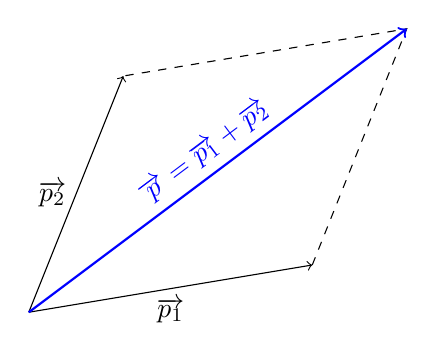
\begin{tikzpicture}[scale=1.2]
		\draw[->] (0,0) -- (3,0.5) node[midway,below]{$\overrightarrow{p_1}$};
		\draw[->] (0,0) -- (1,2.5) node[midway,left]{$\overrightarrow{p_2}$};
		\draw[dashed] (3,0.5) -- (4,3) -- (1,2.5);
		\draw[thick, ->, blue] (0,0) -- (4,3) node[midway,above,rotate=36.87]{$\overrightarrow{p} = \overrightarrow{p_1} + \overrightarrow{p_2}$};
		\end{tikzpicture}
	\end{minipage}
	\begin{minipage}[b]{0.45\textwidth}
		\centering
		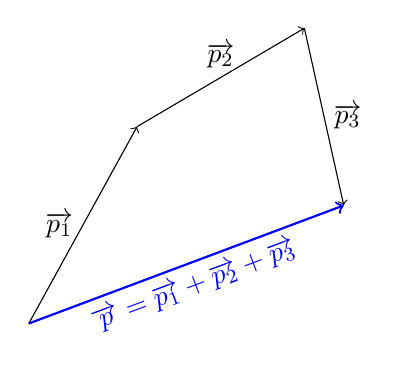
\begin{tikzpicture}[scale=1.25]
		\draw[->] (0,0) -- (1.1,2) node[midway,left]{$\overrightarrow{p_1}$};
		\draw[->] (1.1,2) -- (2.8,3) node[midway,above]{$\overrightarrow{p_2}$};
		\draw[->] (2.8,3) -- (3.2,1.2) node[midway,right]{$\overrightarrow{p_3}$};
		\draw[thick, ->, blue] (0,0) -- (3.2,1.2) node[midway,below,rotate=20.556]{$\overrightarrow{p} = \overrightarrow{p_1} + \overrightarrow{p_2} + \overrightarrow{p_3}$};
		\end{tikzpicture}
	\end{minipage}
\end{figure}

\example{A river flows from south to north with a speed of $2.0 \mps$ and the speed of a boat with respect to the water flow is $5.0 \mps$. (a) Suppose the boat leaves the west bank heading due east, what is the resultant velocity of the boat? (b) If the boat is to reach the exact opposite bank across the river, what is the resultant velocity and in what direction should the boat be headed?}

\sol vector diagrams for resultant velocity of the boat is illustrated below

\begin{figure}[ht]
	\centering
	\begin{minipage}[b]{0.45\textwidth}
		\centering
		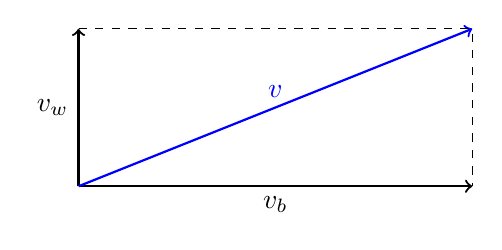
\begin{tikzpicture}
		\draw[thick,->] (0,0) -- (0,2) node[midway,left]{$v_w$};
		\draw[thick,->] (0,0) -- (5,0) node[midway,below]{$v_b$};
		\draw[thick,blue,->] (0,0) -- (5,2) node[midway,above]{$v$};
		\draw[dashed] (0,2) -- (5,2) -- (5,0);
		\end{tikzpicture}
		
		\vspace*{20pt}
		
		(a) boat heading due south
	\end{minipage}
	\begin{minipage}[b]{0.45\textwidth}
		\centering
		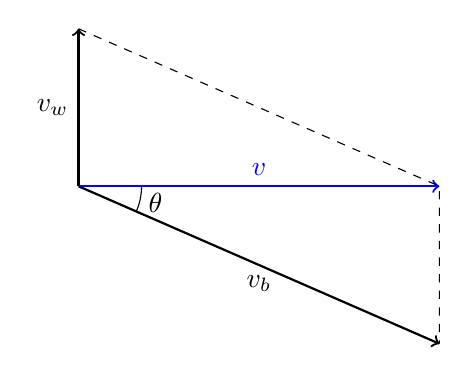
\begin{tikzpicture}
		\draw[thick,->] (0,0) -- (0,2) node[midway,left]{$v_w$};
		\draw[thick,->] (0,0) -- (4.583,-2) node[midway,below]{$v_b$};
		\draw[thick,blue,->] (0,0) -- (4.583,0) node[midway,above]{$v$};
		\draw[dashed] (0,2) -- (4.583,0) -- (4.583,-2);
		\draw (0.8,0) arc(0:-23.58:0.8);
		\node at (-12:1) {$\theta$};
		\end{tikzpicture}
		
		(b) boat aiming at exact opposite bank
	\end{minipage}
\end{figure}

\begin{compactitem}
	\item[(a)] magnitude of resultant velocity: $v = \sqrt{v_b^2 + v_w^2} = \sqrt{5.0^2 +2.0^2} \approx 5.4 \mps$
	
	in this case, the boat reaches the opposite bank in shortest time but will drift downstream
	
	\item[(b)] magnitude of resultant velocity: $v = \sqrt{v_b^2 + v_w^2} = \sqrt{5.0^2 -2.0^2} \approx 4.6 \mps$
	
	in this case, the boat reaches the opposite bank in shortest distance
	
	but the boat is headed slightly upstream: $\theta = \sin^{-1} \frac{v_w}{v_b} = \sin^{-1}\frac{2.0}{5.0} \approx 24^\circ$ \eoe
\end{compactitem}



\subsubsection{resolving vectors}

one can also resolve a single vector into two (or more) components
\footnote{This depends on the number of dimensions of space we are working with.}

\begin{wrapfigure}{R}{0.36\textwidth}
	\vspace{-18pt}
	\begin{center}
		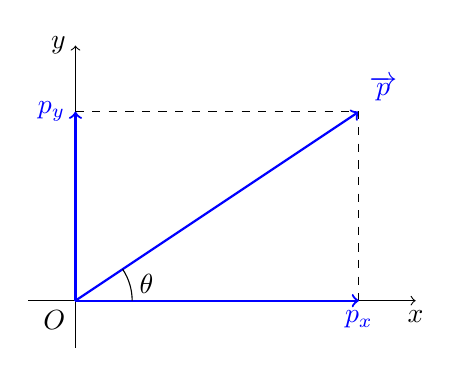
\begin{tikzpicture}[scale=1.2]
		\draw[->] (-.5,0) -- (3.6,0) node[below]{$x$};
		\draw[->] (0,-.5) -- (0,2.7) node[left]{$y$};
		\draw[thick, ->, blue] (0,0) node[below left]{\textcolor{black}{$O$}} -- (3,2) node[above right]{$\overrightarrow{p}$};
		\draw[dashed] (0,2) -- (3,2) -- (3,0);
		\draw[thick, ->, blue] (0,0) -- (0,2) node[left]{$p_y$};
		\draw[thick, ->, blue] (0,0) -- (3,0) node[below]{$p_x$};
		\draw (0:0.6) arc [radius=0.6, start angle=0, end angle= 33.7] node[midway,right]{$\theta$};
		\end{tikzpicture}
	\end{center}
	\vspace{-25pt}
\end{wrapfigure}

let's place a general 2D vector $\overrightarrow{p}$ in Cartesian coordinates

vector $\overrightarrow{p}$ can be split into two perpendicular components

\titem a horizontal component $p_x$

\titem a vertical component $p_y$

if $\overrightarrow{p}$ forms an angle $\theta$ to the $x$-axis, then:

{
	\centering
	
	$p_x = p \cos \theta, \quad p_y = p \sin \theta$
	
	$p = |\overrightarrow{p}| = \sqrt{p^2_x + p^2_y}, \quad\tan \theta = \frac{p_y}{p_x}$
	
}


\example{A force of 3.0 N towards east and a force of 2.0 N towards 30$^\circ$ north of east act on an object. Find the magnitude and the direction of the resultant force.}


\sol suppose an arrow of length 1 cm represents a force of 1 N

one can draw a \emph{scale diagram} with a ruler and a protractor as shown

\begin{figure}[ht]
	\centering
	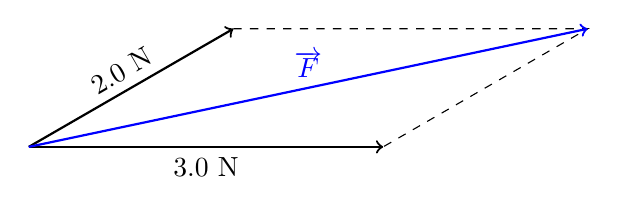
\begin{tikzpicture}[scale = 1.5]
	\draw[thick,->] (0,0) -- (3,0) node[midway,below]{3.0 N};
	\draw[thick,->] (0,0) -- ++ (30:2) node[midway,above,rotate=30]{2.0 N};
	\draw[dashed] (30:2) --++ (3,0) --++ (-150:2);
	\draw[thick,blue,->] (0,0) -- (4.732,1) node[midway, above]{$\overrightarrow{F}$};
	\end{tikzpicture}
\end{figure}

one can find length of the resultant vector is about 4.8 cm

also it forms an angle of about 12$^\circ$ to the 3.0 N force

so resultant force is of 4.8 N acting towards 12$^\circ$ north of east

alternatively, one can find components of the resultant as the sum of individual components

{
	\centering
	
	$F_x = 3.0 + 2.0 \cos 30^\circ \approx 4.73 \text{ N}, \quad F_y = 2.0\sin30^\circ = 1.0 \text{ N}$
	
}

magnitude and direction of the resultant can then be found from its components

{
	\centering
	
	$F = \sqrt{F_x^2 + F_y^2} = \sqrt{4.73^2 + 1.0^2} \approx 4.84 \text{ N}, \theta = \tan^{-1}\frac{F_y}{F_x} = \tan^{-1}\frac{1.0}{4.73} \approx 11.9^\circ$
	
}

this of course agrees with scale diagram method, but resolving gives more precise results \eoe

\begin{wrapfigure}{r}{0.5\textwidth}
	\vspace*{-10pt}
	\centering
	\begin{tikzpicture}[scale=1.1]
	\draw[thick] (0,0) -- (30:5) -- ++(0,-2.5) -- cycle;
	\draw[thick] (0.8,0) arc(0:30:0.8);
	\node at (15:1) {$\theta$};
	\draw[thick] (30:2.5) -- ++(120:1) -- ++(30:1) -- ++(-60:1);
	\draw[thick] (-1,0) -- (5,0);
	\draw[thick,->] (2.348,1.933) --++ (0,-1.6) node[right,pos=0.7]{$W$};
	\draw[thick,blue,->] (2.348,1.933) --++ (210:0.8) node[left]{$W_\parallelslant$};
	\draw[thick,blue,->] (2.348,1.933) --++ (-60:1.38564) node[right]{$W_\perp$};;
	\draw[dashed] (2.348,1.933) ++ (210:0.8) --++ (-60:1.38564) --++ (30:0.8) ;
	\end{tikzpicture}
	\vspace*{-16pt}
\end{wrapfigure}


\example{A box of weight $W=20.0 \text{ N}$ is resting on an inclined slope at 30$^\circ$ to the horizontal. Find the components of weight parallel to the slope and normal to the slope.}\label{ex:comp-of-W}

\sol the vector diagram is shown

component of weight parallel to slope: $W_\parallelslant = W\sin\theta = 20.0\times \sin30^\circ = 10.0 \text{ N}$

component of weight normal to slope: $W_\perp = W\cos\theta = 20.0\times \cos30^\circ \approx 17.3 \text{ N}$ \eoe


 
\subsection{uncertainties}
 
physics is a practical science, any law of physics must be evidenced by experimental facts

any meaningful physical quantity is measured either directly or indirectly

but repeated readings may not give a consistent value, instead they show a \emph{spread} of data

\keypoint{uncertainty} gives the \emph{range} of values in which \emph{true value} of the measurement is asserted to lie

measurement of a particular quantity is usually reported as $x \pm \Delta x$, where reported value $x$ is the average of repeated readings, and $\Delta x$ is its uncertainty

\subsubsection{absolute uncertainty}

$\Delta x$ measures the size of the range of values where true value probably lies

therefore $\Delta x$ is called the \keypoint{absolute uncertainty}\index{uncertainty!absolute uncertainty}

\cmt absolute uncertainty $\Delta x$ carries the same unit as quantity $x$

\cmt absolute uncertainty can be worked out from \emph{range} of readings

range of a data set ${x_1, x_2, x_3, \cdots}$ is the difference between greatest and smallest value

absolute uncertainty is given by: $\boxed{\Delta x = \frac{1}{2}\left(x_\tmax-x_\tmin\right)}$

\cmt absolute uncertainty is usually kept to one significant figure only
\footnote{In some cases where the uncertainty of a quantity is not stated explicitly, the uncertainty is indicated by the number of significant figures in the stated value. If the height of a person is measured to be 1.75 m, this means the first two digits (1 and 7) are certain, while the last digit (5) is uncertain.
	
When you add or subtract numbers, the number of significant figures is determined by the location of the decimal place. For example, $1.11+\underline{4.2}+0.563=5.873$, the result should be written as $5.9$. When you multiply or divided numbers, the result can have no more significant figures than the term with the fewest significant figures. For example, $1.35\times462\times\underline{0.27} = 168.399$, the result should be written as 170.

However, in AS \& A-Level physics, apart from the problems regarding uncertainties, it is allowed to give one more significant figure that what is required. So in other sections of my notes where we do not keep track of the uncertainties, I could be a bit sloppy with the issue of significant figures when numerical values are worked out.}

since $\Delta x$ indicates where the readings start to get problematic

measured quantity $x$ is kept to the same decimal place as $\Delta x$

for example, if value for the speed of an athlete is found to be $v=(8.16\pm0.27)\mps$, the result, to an appropriate number of significant figures, should be kept as: $v=(8.2\pm0.3) \mps$.



\subsubsection{fractional \& percentage uncertainty}

ratio of absolute uncertainty to reported value, i.e., $\frac{\Delta x}{x}$, gives the \keypoint{fractional uncertainty}

recording this ratio as a percentage number, this is known as the \keypoint{percentage uncertainty}\index{uncertainty!percentage uncertainty}

\cmt fractional and percentage uncertainty have no unit

\cmt $\frac{\Delta x}{x}$ gives relative measure of spread of data, so it is also called the relative uncertainty

\example{A students measures the diameter of a cylindrical bottle with a vernier calliper. The measurements are taken from several different positions and along different directions. The readings she obtained are: 4.351 cm, 4.387 cm, 4.382 cm, 4.372 cm, 4.363 cm. What is the percentage uncertainty of her measurements?}

\sol average value: $d = \frac{1}{5}(4.351+4.387+4.382+4.372+4.363) = 4.371 \text{ cm}$

absolute uncertainty: $\Delta d = \frac{1}{2}\left(d_\tmax-d_\tmin\right) = \frac{1}{2}(4.387-4.351) = 0.036 \text{ cm}$

result of measurement should be recorded as: $ d = 4.37 \pm 0.04 \text{ cm}$

percentage uncertainty: $\frac{\Delta d}{d} = \frac{0.036}{4.371} \approx 0.082\%$   \eoe




\subsubsection{propagation of uncertainties}\index{uncertainty!propagation}

in many situations, the quantity that we want to find cannot be measured directly

the quantity of interest has to be computed from other quantities

uncertainty of this calculated quantity would depend on two things:

\titem uncertainties of the raw data from which it is calculated,

\titem how calculated quantity is related to those original quantities

\vspace*{\baselineskip}

suppose quantities $A$ and $B$ are two measurables with uncertainty $\Delta A$ and $\Delta B$ 

$X$ is a quantity to be computed by taking their sum, difference, product or quotient

to evaluate uncertainty in $X$, we estimate the worst scenario, i.e., the greatest deviation from its reported value

\subsubsection*{addition: $S=A+B$}

$S_\tmax = A_\tmax + B_\tmax = (A + \Delta A) + (B + \Delta B) = (A+B) + (\Delta A + \Delta B)= S + (\Delta A + \Delta B) \RA \boxed{\Delta S = \Delta A + \Delta B}$

\subsubsection*{subtraction: $D=A-B$}

$D_\tmax = A_\tmax - B_\tmin = (A + \Delta A) - (B - \Delta B) = (A-B) + (\Delta A + \Delta B)= D + (\Delta A + \Delta B) \RA \boxed{\Delta D = \Delta A + \Delta B}$

\subsubsection*{multiplication: $P=AB$}

$P_\tmax = A_\tmax B_\tmax = (A + \Delta A)(B + \Delta B) = AB + B\Delta A + A\Delta B + \Delta A \Delta B \RA \Delta P =  B\Delta A + A\Delta B + \Delta A \Delta B$

divide both sides by $P=AB$, we get
\begin{equation*}
\frac{\Delta P}{P} = \frac{\Delta A}{A} + \frac{\Delta B}{B} + \frac{\Delta A}{A}\cdot\frac{\Delta B}{B} \RA \boxed{\frac{\Delta P}{P} = \frac{\Delta A}{A} + \frac{\Delta B}{B}}
\end{equation*}

percentage uncertainty of a measurable is usually a few percent, so $\frac{\Delta A}{A}\cdot\frac{\Delta B}{B} \approx 0$

so this piece is dropped from the last expression

\subsubsection*{division: $Q=\frac{A}{B}$}

one can show that $\boxed{\frac{\Delta Q}{Q} = \frac{\Delta A}{A} + \frac{\Delta B}{B}}$

the derivation is left as an exercise for the reader

\subsubsection*{power \& roots: $Q=A^l B^m C^n\cdots$}

percentage uncertainty in $Q$ is: $\frac{\Delta Q}{Q} = l\frac{\Delta A}{A} + m\frac{\Delta B}{B} + n\frac{\Delta C}{C} +\cdots$

this can be thought of as a generalization for multiplication and division operations

the proof is also left as an exercise to the reader

\subsubsection*{brief summary}

\begin{ilight}
	-- for addition and subtraction, \emph{absolute uncertainties} add up
	
	-- for multiplication, division and powers, \emph{percentage uncertainties} add up
	
\end{ilight}

\cmt notice that uncertainties always add

\example{The resistance of a resistor is measured in an experiment. The current through the resistor is $1.8\pm0.1$ A and the potential difference across is $7.5\pm 0.2$ V. What is the resistance of the resistor and its uncertainty?}

value of resistance: $R=\frac{V}{I} = \frac{7.5}{1.8} \approx 4.17  \text{ }\Omega$

percentage uncertainty in resistance: $\frac{\Delta R}{R} = \frac{\Delta V}{V} + \frac{\Delta I}{I} = \frac{0.2}{7.5} + \frac{0.1}{1.8} \approx 8.2 \%$

absolute uncertainty in resistance: $\Delta R = 8.2\% \times 4.17 \approx 0.34 \text{ }\Omega$

so we find resistance of the resistor: $R = 4.2 \pm 0.3  \text{ }\Omega$ \eoe

\example{The density of a liquid is found by measuring its mass and its volume. The following is a summary of the measurements: $\text{mass of empty beaker} = (20\pm1)\text{g}$, $\text{mass of beaker and liquid} = (100\pm1)\text{g}$,  and $\text{volume of liquid} = (10.0\pm0.5)\text{cm}^3$. What is the density of this liquid and the uncertainty in this value?}

\sol mass of liquid: $m = m_2 - m_1 = 100 -20 = 80 \text{ g}$

uncertainty in mass: $\Delta m = \Delta m_2 + \Delta m_1 = 1 + 1 = 2 \text{ g}$

density of liquid: $\rho = \frac{m}{V} = \frac{80}{10.0} = 8.00 \text{ g cm}^{-3}$

percentage uncertainty in density: $\frac{\Delta \rho}{\rho} = \frac{\Delta m}{m} + \frac{\Delta V}{V} = \frac{2}{80} + \frac{0.5}{10.0} = 7.5 \%$

absolute uncertainty in density: $\Delta \rho = 7.5\% \times 8.00 = 0.60 \text{ g cm}^{-3}$

so density of this liquid is recorded as: $\rho = 8.0 \pm 0.6 \text{ g cm}^{-3}$ \eoe

\example{The period of simple pendulum is given by $T=2\pi\sqrt{\frac{L}{g}}$. In an experiment, the length of string is measured to be $L=100.0\pm0.5$ cm, and the time taken for 10 full oscillations is $t=20.0\pm 0.2$ s. What is the value for acceleration of free fall $g$ and its uncertainty?}

\sol period of one oscillation: $T = \frac{1}{10}t = 2.00 \pm 0.02 \text{ s}$

let's rearrange $T=2\pi\sqrt{\frac{L}{g}}$ into $g = \frac{4\pi^2L}{T^2}$

acceleration of free fall: $g = \frac{4\pi^2 \times 100.0}{2.00^2} \approx 987 \text{ cm s}^{-2}$

\eqyskip percentage uncertainty: $\frac{\Delta g}{g} = \frac{\Delta L}{L} + 2\frac{\Delta T}{T} = \frac{0.5}{100.0} + 2\times\frac{0.02}{2.00} = 2.5\%$ \footnote{Starting from the formula $T=2\pi\sqrt{\frac{L}{g}}$, it is attempting to write $\frac{\Delta T}{T} = \frac{1}{2}\frac{\Delta L}{L} + \frac{1}{2}\frac{\Delta g}{g}$. But this would mean that $T$ is a calculated quantity whose uncertainty is determined by the uncertainty in $L$ and the uncertainty in $g$, which is incorrect. The right way to do it is to rearrange the formula so that calculated quantity of interest is made the subject of the working equation, the propagation of uncertainties then becomes explicit.}

absolute uncertainty: $\Delta g = 2.5\% \times 987 \approx 24.7 \text{ cm s}^{-2}$

so result of this measurement is: $ g = 990 \pm 20 \text{ cm s}^{-2}$ \eoe




\subsection{measurement errors}

difference between the measured value and the true value is called \keypoint{error}

total error is usually a combination of two components: systematic error and random error

\subsubsection{systematic \& random errors}

\begin{ilight}
	\keypoint{systematic errors} cause the readings to be greater or smaller than the true value by the same amount\index{systematic error}
\end{ilight}

\cmt faulty equipments, biased observers, calibration errors could produce systematic errors

examples of systematic errors include:

\titem a vernier calliper does not read zero when fully closed, this introduces \keypoint{zero error}

\titem one always reads a measuring cylinder from a higher angle, this introduces \keypoint{parallax error}

\titem spring of force meter becomes weaker over time, so force meter always gives overestimates

\cmt systematic errors can be reduced by using better equipments or methods

\titem one can check for zero error before taking readings with a micrometer

\titem one can \emph{calibrate} a balance with a known mass before using it to measure mass of an object



\begin{ilight}
	\keypoint{random errors} cause the readings to fluctuate above or below the actual value\index{random error}
\end{ilight}


\cmt deviations caused by random error are unpredictable

\cmt insensitive equipments, lack of observer precision, changes in environment, imprecise definitions could produce random errors

examples of causes of random errors include:

\titem \keypoint{human reaction errors} when measuring a time quantity on a stop-watch

\titem electronic noise due to thermal vibrations of atoms when measuring an electric current

\titem when measuring length of a crack, different people could pick different end points

\cmt random errors can be reduced by averaging the results from repeated measurements

for example, diameter of a sphere can be measured along different directions and averaged

\cmt random errors can also be reduced by using better equipment and better technique

for example, time for an object to fall can be measured with a light gate, instead of a stopwatch

\begin{wrapfigure}{r}{0.5\textwidth}
	\centering
	\vspace*{-15pt}
	\begin{tikzpicture}[xscale=1,yscale=0.9]
	\draw[<->] (0,5) node[left]{$I$} -- (0,0) -- (6,0) node[below]{$V$};
	\node[blue] at (1.5,0.4) {$\times$};
	\node[blue] at (2.5,1.6) {$\times$};
	\node[blue] at (3.6,2.3) {$\times$};
	\node[blue] at (4.8,3.4) {$\times$};
	\node[blue] at (5.6,4.7) {$\times$};
	\draw[thick,red] (0.5,-0.4) --++ (5.5,5.2);
	\end{tikzpicture}
	\vspace*{-15pt}
\end{wrapfigure}

\example{An experiment is carried out to measure the resistance of a metallic resistor, which is known to be constant throughout the experiment. A set of readings for voltage $V$ across the resistor and the corresponding current $I$ are obtained. A graph of $I$ against $V$ is plotted as shown. What can you say about the errors of the experiment?}

\sol one can first draw a \emph{best fit line} to see the distribution of data points

constant resistance means $I$ should be directly proportional to $V$

so the best fit should be a straight line through the origin

but the best fit does not pass through origin, so there exists systematic error

also data points scatter above and below the best fit, so random errors are present \eoe


\subsubsection{accuracy \& precision}

to analyse the result of an experiment, two important aspects are accuracy and precision

\begin{ilight}
	measurement is said to be \keypoint{accurate} if the result is close to the true value\index{accuracy}
\end{ilight}

\begin{ilight}
	measurement is said to be \keypoint{precise} if repeated readings are close to each other\index{precision}
\end{ilight}

\begin{figure}[htp]
	\centering
	\begin{minipage}{0.32\textwidth}
		\centering
		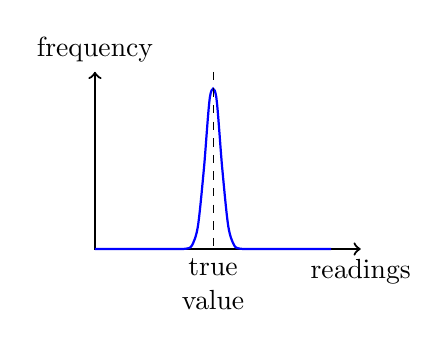
\begin{tikzpicture}[scale = .75]
		\draw [thick, <->] (4.5,0) node[below]{readings} -- (0,0) --(0,3) node[above]{frequency};
		\draw [thick,blue,domain=0:4,samples=40,smooth,variable=\x] plot (\x, {2.8*exp(-30*(\x-2)^2)});
		\draw[dashed] (2,3) -- (2,0) node[below,align=center,execute at begin node=\setlength{\baselineskip}{1.2em}]{true\\value};
		\end{tikzpicture}
		
		(a) precise and accurate
	\end{minipage}\hfil
	\begin{minipage}{0.32\textwidth}
		\centering
		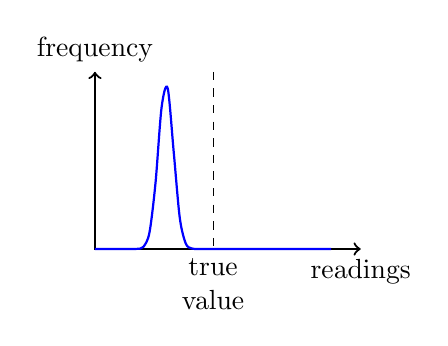
\begin{tikzpicture}[scale = .75]
		\draw [thick, <->] (4.5,0) node[below]{readings} -- (0,0) --(0,3) node[above]{frequency};
		\draw [thick,blue,domain=0:4,samples=40,smooth,variable=\x] plot (\x, {2.8*exp(-30*(\x-1.2)^2)});
		\draw[dashed] (2,3) -- (2,0) node[below,align=center,execute at begin node=\setlength{\baselineskip}{1.2em}]{true\\value};
		\end{tikzpicture}
		
		(b) precise but not accurate
	\end{minipage}\hfil
	\begin{minipage}{0.32\textwidth}
		\centering
		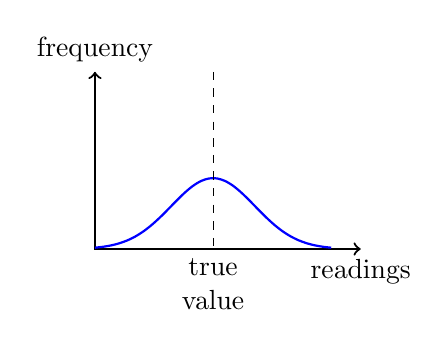
\begin{tikzpicture}[scale = .75]
		\draw [thick, <->] (4.5,0) node[below]{readings} -- (0,0) --(0,3) node[above]{frequency};
		\draw [thick,blue,domain=0:4,samples=30,smooth,variable=\x] plot (\x, {1.2*exp(-1*(\x-2)^2)});
		\draw[dashed] (2,3) -- (2,0) node[below,align=center,execute at begin node=\setlength{\baselineskip}{1.2em}]{true\\value};
		\end{tikzpicture}
		
		(c) accurate but not precise
	\end{minipage}
	
	\caption*{distribution of readings with different precision and accuracy}
\end{figure}

\cmt accuracy of a measurement is closely related to systematic errors

large systematic errors mean the results must be inaccurate

\cmt precision of a measurement is closely related to random errors

large random errors cause repeated readings to spread, so the result must be imprecise

\cmt precision is usually indicated by the percentage uncertainty of the measurement

similarly, precision is also indicated by the number of significant figures in a measurement

for example, metre rule has a precision of 0.1 cm, while micrometer has a precision of 0.001 cm


\example{The value for the acceleration of free fall is determined in an experiment. The result is reported to be $g=14\pm5 \mpss$. Is this result accurate? Is it precise?}

\sol true value for $g$ is around $9.8\mpss$

stated value is not close to the true value, so the result is not accurate

percentage uncertainty in this result is $\frac{5}{14}\approx 36\%$, which is quite large

so the result is not precise either \eoe



\ifthenelse{\includequestions=1}{
	
\subsection{end-of-chapter questions}

\subsubsection*{SI units}

\question{What are the SI base units of (a) density, (b) pressure, (c) energy, (d) electric charge?}

\question{For a substance of mass $m$, the heat energy $Q$ needed to change its temperature by $\Delta T$ is given by: $Q = cm\Delta T$. Find the SI base units of the constant $c$.}

\subsubsection*{dimensional analysis}

\question{The resistive force $F$ on a metal ball falling at low speeds in water is given by the equation $F = krv$, where $r$ is the radius of the metal ball, $v$ is its speed and $k$ is a constant.
	Find the base units of $k$ in the SI system.}

\question{The speed of sound in air can be given by $c=\sqrt{\frac{\gamma p}{\rho}}$, where $p$ is the pressure of the air and $\rho$ is the air density. Show that $\gamma$ is unit free.}

\question{The effective power output from a wind turbine is given by the equation $P = \frac{1}{2} \eta \rho A v^n$, where $\rho$ is the air density, $A$ is the area of the turbine blades, and $v$ is the wind speed. Given that $\eta$ is a constant with no units, what is the value of $n$?}

\subsubsection*{vector algebra}

\question{An aircraft, which has a speed of $35 \mps$ in still air, is flying from south to north at a speed of $32 \mps$ with respect to a stationary observer on the ground. Find the magnitude and the possible directions of wind velocity.}

\question{Three forces of 5.0 N, 12 N and 13 N act at one point on an object. The angles at which the forces act can vary. What is the maximum and the minimum resultant force?}

\subsubsection*{propagation of uncertainties}

\question{A thermometer can measure to a precision of $0.5 ^\circ$C , what is the temperature rise from $20.0 ^\circ$C to $50.0 ^\circ$C and its uncertainty?}

\question{The radius of a sphere is measured to be $5.0$ cm with an uncertainty of 1\%. What is the volume of this sphere and the uncertainty? (Volume of a sphere is given by: $V=\frac{4}{3}\pi R^3$.)}

\question{The power radiated from a star of radius $R$ and surface temperature $T$ is given by the formula: $P = 4\pi \sigma R^2 T^4$, where $\sigma$ is the Stefan–Boltzmann constant known to have the value of $5.67\times10^{-8} \text{ W m}^{-2} \text{ K}^{-4}$. If the sun is measured to have a surface temperature of $5800 \pm 200 \text{ K}$ and a diameter of $(1.40\pm0.03)\times10^9 \text{ m}$. (a) Find the radiation power $P$ of the sun and its absolute uncertainty. (b) Suggest which measurement has a larger effect on the uncertainty in $P$.}




}{}